% Prezentacja artykułu (Lab 5): 8 slajdów, do 5 minut.
% Kompilacja: latexmk -pdf presentation.tex. examples.pdf, conditions.pdf i ranking.pdf to kopie z ../article/figures;
% po przegenerowaniu wykresów trzeba je tu skopiować ponownie. Na slajdzie 3 examples.pdf jest przycięty (trim) na dwie
% części ustawione obok siebie, więc po zmianie rysunku trzeba sprawdzić przycięcie.
% Liczby jak w artykule (research/results/, tables/overall.tex); odczyty skanu ze slajdu 7: research/results/gold/*.csv,
% images/inwokacja_0000.png.
\documentclass[aspectratio=169,11pt]{beamer}
\usepackage[T1]{fontenc}
\usepackage[utf8]{inputenc}
\usepackage{polski}
\usepackage{lmodern}
\usepackage{booktabs}
\usepackage{array}
\usepackage{hyperref}

\usetheme{default}
\usecolortheme{seahorse}
\setbeamertemplate{navigation symbols}{}
\setbeamertemplate{footline}[frame number]
\setbeamersize{text margin left=1cm,text margin right=1cm}
\definecolor{akcent}{rgb}{0.2,0.2,0.7}
\definecolor{blad}{rgb}{0.8,0.1,0.1}
\setbeamercolor{block title}{bg=akcent!18,fg=akcent!70!black}
\setbeamercolor{block body}{bg=akcent!6}
\setbeamerfont{block title}{size=\small,series=\bfseries}

% Wąska kolumna z etykietą po lewej, bez justowania; bez \leavevmode kolor przesuwa pierwszy wiersz komórki w dół.
\newcolumntype{L}[1]{>{\raggedright\arraybackslash\leavevmode\color{akcent!70!black}}p{#1}}
\newcolumntype{P}[1]{>{\raggedright\arraybackslash}p{#1}}
% Treść ramki o stałej wysokości, żeby sąsiednie ramki miały równą wysokość.
\newenvironment{rowna}[1]{\vspace*{-0.5\baselineskip}\begin{minipage}[t][#1][t]{\linewidth}\vspace{0pt}\raggedright}{\end{minipage}}
\newcommand{\zrodlo}[1]{\par\vfill{\tiny\color{black!65}#1\par}}
\newcommand{\bl}[1]{\textcolor{blad}{#1}}

\title{Ocena silników OCR i~modeli wizyjno-językowych w~rozpoznawaniu tekstu polskiego na danych syntetycznych
  i~rzeczywistych}
\author{Anton Ovod, Maciej Pietras, Marek Siuzdak, Paweł Podgórski}
\institute{Politechnika Lubelska, Wydział Elektrotechniki i~Informatyki}
\date{22.11.2026}

\begin{document}

% 1 --------------------------------------------------------------------------
\begin{frame}[plain]
  \titlepage
\end{frame}

% 2 --------------------------------------------------------------------------
\begin{frame}{Motywacja i~cel pracy}
  \small
  \begin{itemize}
    \item Modele wizyjno-językowe (VLM) uczy się głównie na danych angielskich i~chińskich.
    \item Alfabet polski ma tymczasem dziewięć liter diakrytycznych ({\color{akcent}ą, ć, ę, ł, ń, ó, ś, ź, ż}),
      które od łacińskich różni tylko ogonek, kreska lub kropka.
    \item Dla tureckiego wykazano, że takie litery należą do głównych źródeł błędów odczytu~[1].
    \item Dla polskiego brakuje porównania VLM z~klasycznymi silnikami OCR.
  \end{itemize}
  \begin{block}{Cel}
    Ocenić, jak dokładnie otwarte silniki OCR i~VLM odczytują tekst polski, i~sprawdzić, czy wyniki uzyskane
    na danych syntetycznych przenoszą się na prawdziwe pismo odręczne.
  \end{block}
  \vspace{-2pt}Pytania badawcze:
  \begin{enumerate}
    \setlength{\itemsep}{0pt}
    \item Które narzędzie najdokładniej odczytuje tekst polski?
    \item Czy polskie znaki, długość, kontekst, pismo odręczne i~zniekształcenia zwiększają błąd?
    \item Czy ranking narzędzi na danych syntetycznych jest taki sam jak na skanach rękopisów?
  \end{enumerate}
  \vspace{10pt}
  \zrodlo{[1] Y.~Yılmaz i~in., \emph{Benchmarking OCR and vision-language models for Turkish text recognition},
  IJDAR, Springer, 2026.}
\end{frame}

% 3 --------------------------------------------------------------------------
\begin{frame}{Materiał: zbiór syntetyczny i~skany}
  \begin{columns}[T]
    \begin{column}{0.41\textwidth}
      \footnotesize
      \begin{tabular*}{\linewidth}{@{}l@{\extracolsep{\fill}}r@{}}
        \textcolor{akcent!70!black}{Źródło tekstu} & Obrazy \\
        \midrule
        \emph{Lalka} B.~Prusa, syntetyczne & 2200 \\
        Inwokacja \emph{Pana Tadeusza}, skany & 1968 \\
      \end{tabular*}

      \medskip
      Obrazy z~generatora TRDG~1.8.0: 2 rodzaje pisma $\times$ 11 podkategorii $\times$ 100, 15 czcionek drukowanych i~19 odręcznych. Skany: ten sam tekst
      przepisany ręcznie przez 1968 osób.
    \end{column}
    \begin{column}{0.55\textwidth}
      \footnotesize
      \begin{tabular}{@{}L{2.3cm}P{\dimexpr\linewidth-2.3cm-2\tabcolsep\relax}@{}}
        Kategoria & Podkategorie \\
        \midrule
        Rodzaj pisma & druk, pismo odręczne \\
        Polskie znaki & z~nimi, bez nich \\
        Długość słowa & do 10, ponad 10 znaków \\
        Kontekst & pojedyncze słowo, zdanie (4--8 słów) \\
        Zniekształcenia & brak, rozmycie, obrót, szum, niska rozdzielczość \\
      \end{tabular}
    \end{column}
  \end{columns}

  \vspace{6pt}
  \noindent\makebox[\linewidth][c]{\resizebox{15cm}{!}{%
    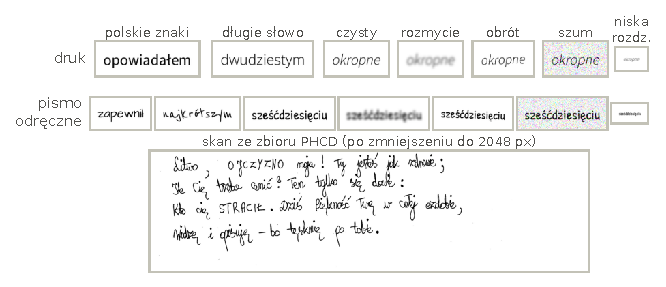
\includegraphics[height=2cm,trim=6 74 7.5 6,clip]{./examples.pdf}\hspace{0.2cm}%
    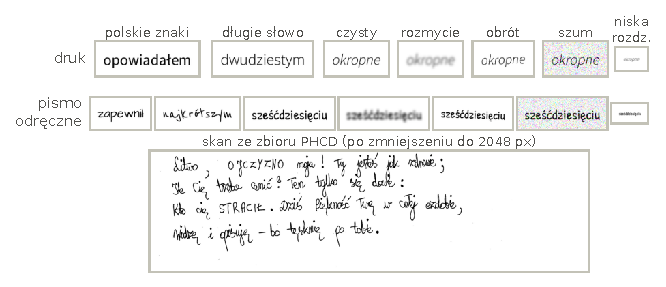
\includegraphics[height=2cm,trim=70 6 35.5 64,clip]{./examples.pdf}}}
  \vspace{8pt}
  \zrodlo{Tekst: \emph{Lalka}, Wolne Lektury (domena publiczna). Skany: baza PHCD Politechniki Lubelskiej
  (Tokovarov i~in., 2020), \url{https://cs.pollub.pl/phcd/}.}
\end{frame}

% 4 --------------------------------------------------------------------------
\begin{frame}{Metody: narzędzia i~miary błędu}
  \begin{columns}[t]
    \begin{column}{0.46\textwidth}
      \begin{block}{7 otwartych narzędzi, bez douczania\vphantom{y}}
        \begin{rowna}{5.3cm}
        \footnotesize
        \begin{tabular}[t]{@{}L{1.9cm}P{\dimexpr\linewidth-1.9cm-2\tabcolsep\relax}@{}}
          VLM & Qwen2.5-VL~7B, InternVL3~8B, DeepSeek-VL2~tiny \\[2pt]
          Model OCR & GOT-OCR2 \\[2pt]
          Klasyczne silniki & PaddleOCR, Tesseract, EasyOCR
        \end{tabular}

        \medskip
        Google Colab, GPU NVIDIA A100; każde narzędzie odczytuje 2200 obrazów syntetycznych i~1968 skanów,
        a~skany w~całości, bez dzielenia na linie.

        \medskip
        \textbf{Polecenie dla VLM:} \emph{,,Extract the Polish text from the image exactly as it appears\ldots''}
        \end{rowna}
      \end{block}
    \end{column}
    \begin{column}{0.51\textwidth}
      \begin{block}{Miary błędu i~analiza}
        \begin{rowna}{5.3cm}
        \footnotesize
        \textbf{CER} (błąd znakowy) $=\min\left(1,\ \dfrac{S+D+I}{N}\right)$\\[2pt]
        $S$, $D$, $I$: znaki podmienione, pominięte i~dopisane przez model; $N$: długość wzorca.
        CER\,=\,0,1 to średnio jeden zły znak na dziesięć. \textbf{WER}: to samo na słowach, dla zdań.

        \setlength{\leftmargini}{1.1em}
        \begin{itemize}
          \setlength{\itemsep}{0pt}
          \item Małe litery, bez interpunkcji; polskie znaki zostają.
          \item Pomyłki wyłącznie diakrytyczne: błędne odpowiedzi zgodne ze wzorcem po usunięciu ogonków i~kresek.
          \item Przedziały ufności 95\%: bootstrap, 1000 prób.
          \item Zgodność rankingów: korelacja Spearmana.
        \end{itemize}
        \end{rowna}
      \end{block}
    \end{column}
  \end{columns}
\end{frame}

% 5 --------------------------------------------------------------------------
\begin{frame}{Wyniki: czynniki utrudniające odczyt}
  \centerline{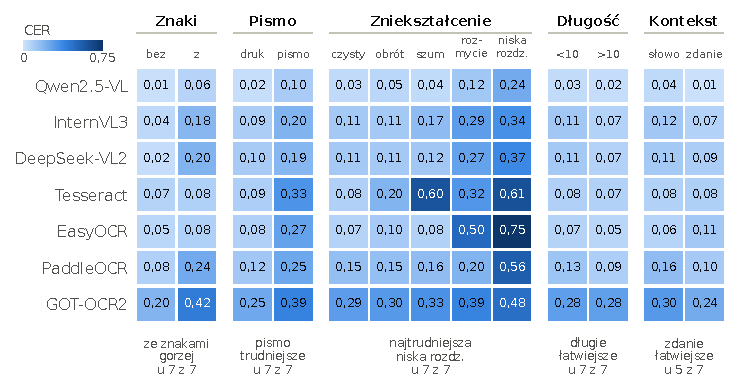
\includegraphics[width=0.78\textwidth]{./conditions.pdf}}
  \footnotesize
  \begin{itemize}
    \item Najdokładniejszy Qwen2.5-VL: CER 0,059, ponad dwukrotnie niższy niż u~kolejnych narzędzi.
    \item Pomyłki wyłącznie diakrytyczne to 26--33\% błędów VLM i~PaddleOCR (Tesseract 3\%).
  \end{itemize}
\end{frame}

% 6 --------------------------------------------------------------------------
\begin{frame}{Wyniki: ranking narzędzi i~walidacja na skanach}
  \centerline{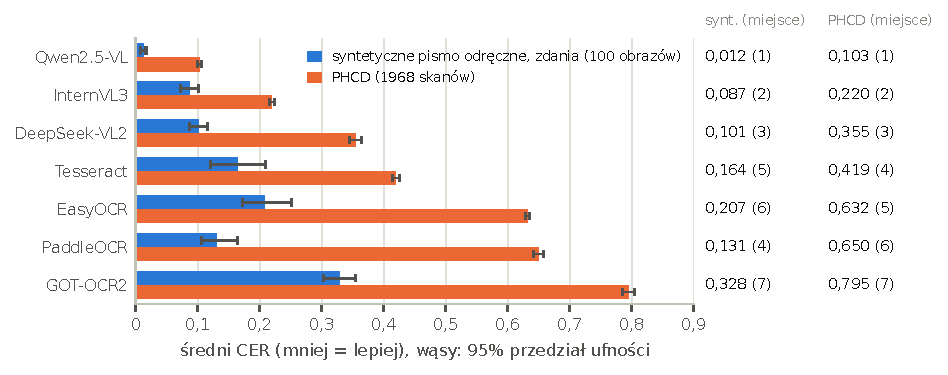
\includegraphics[width=0.84\textwidth]{./ranking.pdf}}
  \small
  \begin{itemize}
    \item Ranking na skanach jest zgodny z~rankingiem na syntetycznych zdaniach odręcznych: $\rho = 0{,}89$,
      $p = 0{,}007$. Zamiany miejsc dotyczą tylko Tesseracta, EasyOCR i~PaddleOCR.
    \item CER na skanach jest co najmniej dwukrotnie wyższy niż na syntetycznych zdaniach odręcznych.
  \end{itemize}
\end{frame}

% 7 --------------------------------------------------------------------------
\begin{frame}{Przykład odczytu skanu PHCD}
  \centerline{\setlength{\fboxsep}{4pt}\fcolorbox{black!30}{white}{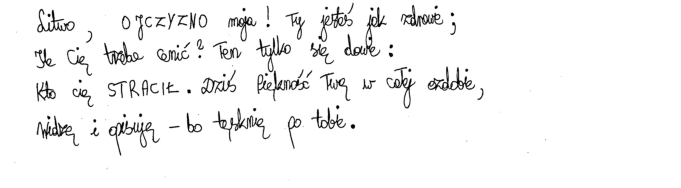
\includegraphics[width=0.58\textwidth]{phcd_scan.png}}}
  \medskip
  \small
  \centering
  \begin{tabular}{@{}lcl@{}}
    \toprule
    & CER skanu & drugi wers \\
    \midrule
    wzorzec & & Ile Cię trzeba cenić? Ten tylko się dowie: \\
    Qwen2.5-VL & 0,11 & \bl{Je} Cię trzeba \bl{ocalić}? Ten tylko się dowie: \\
    InternVL3 & 0,25 & \bl{śle} cię trzeba \bl{emicą}. Ten tylko \bl{ser dawie}: \\
    DeepSeek-VL2 & 0,28 & \bl{Je Cie trobe conic}? Ten \bl{tyko sie dowe}: \\
    GOT-OCR2 & 0,95 & \bl{s it u o} \quad {\footnotesize (cała odpowiedź)} \\
    \bottomrule
  \end{tabular}
\end{frame}

% 8 --------------------------------------------------------------------------
\begin{frame}{Wnioski}
  \small
  \begin{enumerate}
    \setlength{\itemsep}{1pt}
    \item Najdokładniej tekst polski odczytuje Qwen2.5-VL, zarówno na obrazach syntetycznych, jak i~na skanach.
    \item Polskie znaki i~niska rozdzielczość pogarszają wyniki prawie wszystkich narzędzi, a~klasyczne silniki
      najwięcej tracą przy piśmie odręcznym i~zniekształceniach.
    \item Ranking z~danych syntetycznych powtarza się na skanach, więc takie dane wystarczą do wstępnego wyboru
      modelu, choć nie przewidują poziomu błędu.
  \end{enumerate}
  \begin{columns}[t]
    \begin{column}{0.48\textwidth}
      \begin{block}{Elementy nowości}
        \begin{rowna}{2.9cm}
        \footnotesize
        \setlength{\leftmargini}{1.2em}
        \begin{itemize}
          \setlength{\itemsep}{1pt}
          \item Porównanie VLM i~klasycznych silników OCR dla języka polskiego.
          \item Kontrolowany zbiór syntetyczny z~polskimi znakami.
          \item Ocena na 1968 rzeczywistych rękopisach z~bazy PHCD.
          \item Analiza pomyłek wyłącznie diakrytycznych.
        \end{itemize}
        \end{rowna}
      \end{block}
    \end{column}
    \begin{column}{0.48\textwidth}
      \begin{block}{Ograniczenia}
        \begin{rowna}{2.9cm}
        \footnotesize
        \setlength{\leftmargini}{1.2em}
        \begin{itemize}
          \setlength{\itemsep}{1pt}
          \item Obrazy syntetyczne: jedna linia na białym tle.
          \item Na skanach zawsze ten sam tekst, który modele mogły znać z~uczenia.
          \item Tylko 7 narzędzi: korelacja istotna dopiero od $\rho \approx 0{,}79$.
          \item Bez modeli zamkniętych i~ponad 8~mld parametrów.
        \end{itemize}
        \end{rowna}
      \end{block}
    \end{column}
  \end{columns}
\end{frame}

\end{document}
